\documentclass{article}

% if you need to pass options to natbib, use, e.g.:
%     \PassOptionsToPackage{numbers, compress}{natbib}
% before loading neurips_2024


% ready for submission
\usepackage[final]{neurips_2024}


% to compile a preprint version, e.g., for submission to arXiv, add add the
% [preprint] option:
%     \usepackage[preprint]{neurips_2024}


% to compile a camera-ready version, add the [final] option, e.g.:
%     \usepackage[final]{neurips_2024}


% to avoid loading the natbib package, add option nonatbib:
%    \usepackage[nonatbib]{neurips_2024}


\usepackage[utf8]{inputenc} % allow utf-8 input
\usepackage[T1]{fontenc}    % use 8-bit T1 fonts
\usepackage{hyperref}       % hyperlinks
\usepackage{url}            % simple URL typesetting
\usepackage{booktabs}       % professional-quality tables
\usepackage{amsfonts}       % blackboard math symbols
\usepackage{nicefrac}       % compact symbols for 1/2, etc.
\usepackage{microtype}      % microtypography
\usepackage{xcolor}         % colors

\usepackage{amsmath}
\usepackage{amsfonts}
\usepackage{amssymb}
\usepackage{mathtools}

\usepackage{titlesec}

\usepackage{subcaption}

\usepackage{float}



\setcounter{secnumdepth}{4}

\titleformat{\paragraph}
{\normalfont\normalsize\bfseries}{\theparagraph}{1em}{}
\titlespacing*{\paragraph}
{0pt}{3.25ex plus 1ex minus .2ex}{1.5ex plus .2ex}



\title{2024/25 PHYS4036 MLiS2 Project Report}

\author{%
  Sam Tam \\
  School of Physics and Astronomy\\
  University of Nottingham\\
  Nottingham, NG7 2RD \\
  \texttt{ppxst5@nottingham.ac.uk}
}


\begin{document}


\maketitle


\begin{abstract}
  This project aims to develop machine learning models to predict the speed and steering angle of images captured by Raspberry Pi cars. The project is divided into two parts: an online challenge and a live test. Models with convolutional and fully connected layers were developed using transfer learning. They ranked first in the online challenge and demonstrated strong performance. In the live test, the model completed 70\% of the tasks, including flawless lane following and stop-on-object, though some challenges remain. Future studies could focus on enhancing data collection for better generalisability.
\end{abstract}

\section{Introduction}
Autonomous driving has rapidly advanced in the field of artificial intelligence (AI). Numerous companies have been founded with the goal of developing reliable self-driving systems \citep{Law_2023}. Hands-on experience is valuable for learning real-word AI applications.

PiCar \citep{SunFounder} is a small robot car equipped with an onboard camera to capture forward-facing perspective of the car's environment, and a Raspberry Pi (RPi) single-board computer \citep{RaspberryPi} for real-time computation. The captured image frames can be used as input to machine learning models running on the RPi that predict control signals, including steering angle and speed, of the car.

This project is divided into two phases: an online challenge and a live test. In the online challenge, models trained on provided data predicted the car's steering angle and speed of a given image. In the live test, models trained on self-collected data were deployed to the PiCar to complete a variety of tasks to assess the model's performance.


\section{Methods}
In both phases of the project — the online challenge and the live test — the objective was to predict the PiCar's steering angle and speed from images captured by its onboard camera. Both control signals were normalised to the range \([0, 1]\) using the following formulas \citep{Kaggle}:

\begin{equation}
  \text{angle}_{\text{norm}} = \frac{\text{angle} - 50}{80}
  \quad \text{where } \text{angle} \in [90 - 40, 90 + 40] = [50, 130]
\end{equation}

\begin{equation}
  \text{speed}_{\text{norm}} = \frac{\text{speed} - 0}{35}
  \quad \text{where } \text{speed} \in [0, 100]
\end{equation}

The normalised angles were restricted to steps of \(1/16 = 0.0625\), resulting in 17 possible angle values. 0 represents fully left, and 1 represents fully right.



\subsection{Online challenge}

The online challenge was assessed by the mean squared error (MSE) of a test dataset's private leaderboard, where a lower value indicated better model performance.

The steering angle models and the speed models were trained separately, to reduce the complexity of data preprocessing and modelling.

\subsubsection{Training data}

There were 13.8k RGB images of resolution 240 x 320 provided with the corresponding normalised labels \citep{Kaggle}. The dataset was noisy and included inaccurate and missing labels, and invalid image files. Figure \ref{fig:inaccurate_label} shows some examples of inaccurate labelling.

\begin{figure}[h]
  \centering
  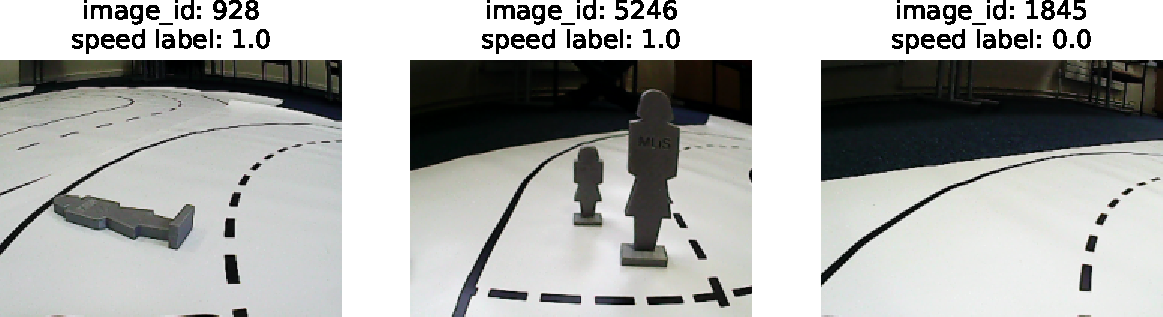
\includegraphics[width=0.8\textwidth]{figures/inaccurate_label.pdf}
  \caption{Examples of inaccurate labels in the dataset.}
  \label{fig:inaccurate_label}
\end{figure}

\paragraph{Data cleaning}
I cleaned the dataset using a script that removed faulty files and ensured labels' validity and completeness. I also manually inspected data that were wrongly classified by the model.

\paragraph{Data distribution}
I visualised the data distribution in Figure \ref{fig:angle_speed_distribution}. It shows that the distribution of steering angles is left-skewed and non-uniform, and the distribution of speeds is imbalanced, roughly 25:75.

\begin{figure}[h]
  \centering
  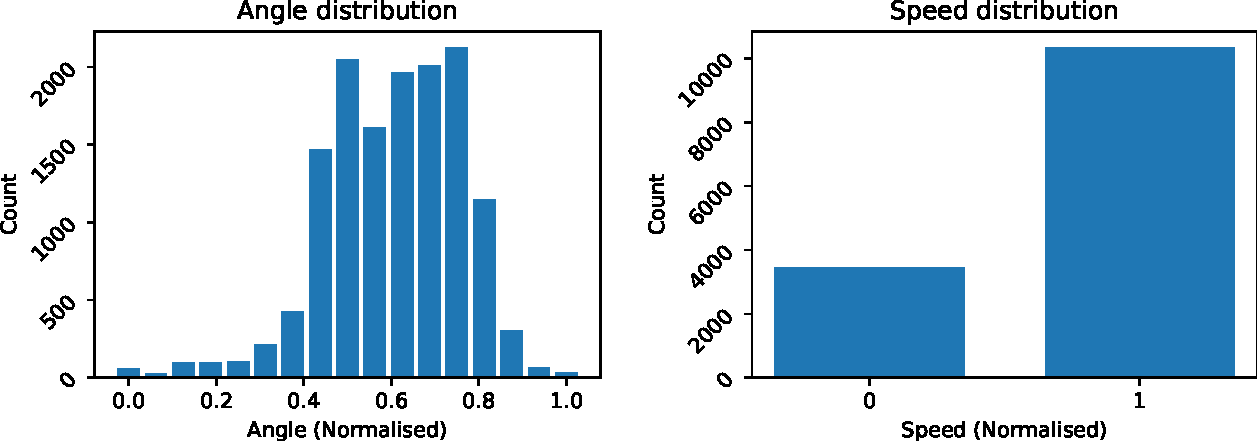
\includegraphics[width=0.9\textwidth]{figures/angle_speed_distribution.pdf}
  \caption{Distribution of steering angles and speeds in the dataset.}
  \label{fig:angle_speed_distribution}
\end{figure}

\paragraph{Training set and test set}
\label{sec:train_test_split}
The data were split into training set and test set, with a ratio of 0.85 : 0.15, using explicitly defined random seeds to assure the ratio between classes in both sets was approximately the same.

\paragraph{Data balancing}
Data balancing was only applied to the training set.

Given the severe class imbalance in steering angle, I applied a combination of oversampling and undersampling to the dataset, leading to a ratio between a minority and a majority class of approximately 0.22 : 0.78. After some experimenting, this ratio yielded the best to avoid overfitting from oversampling and underfitting from excessive undersampling.

I left the speed dataset unchanged and used weighted loss to address the class imbalance instead, as it was not highly imbalanced.

Figure \ref{fig:angle_speed_distribution_balanced} shows the distribution of steering angles and speeds after balancing.

\begin{figure}[h]
  \centering
  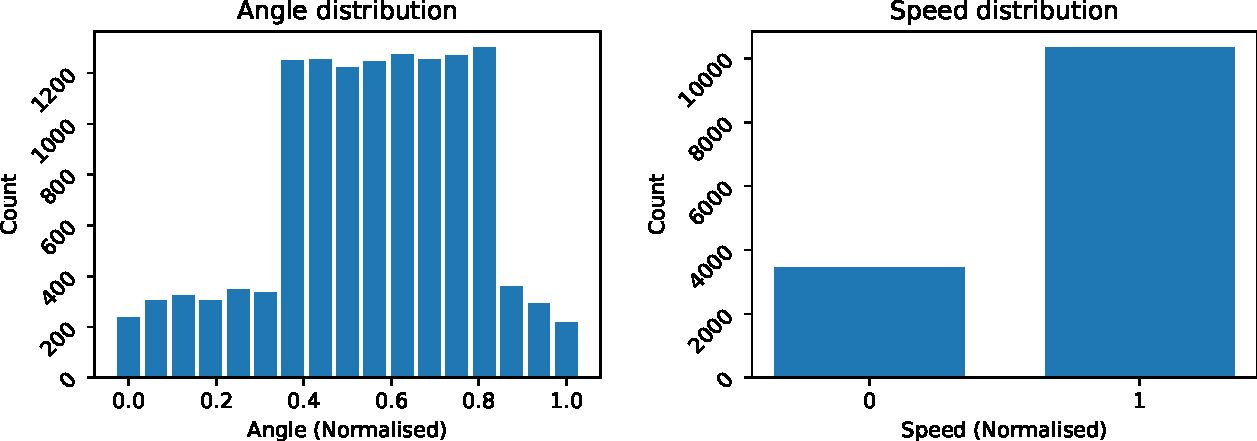
\includegraphics[width=0.9\textwidth]{figures/angle_speed_distribution_balanced.pdf}
  \caption{Distribution of steering angles and speeds after balancing.}
  \label{fig:angle_speed_distribution_balanced}
\end{figure}

\paragraph{Data augmentation}
\label{sec:data_augmentation}
To mimic real-world conditions, I augmented the training data in lighting and camera angle variations. The augmentations were applied randomly, as listed in Table \ref{tab:data_augmentation}. Figure \ref{fig:augmentation} shows some samples of the augmentation.

\begin{table}[H]
  \centering
  \renewcommand{\arraystretch}{1.2}
  \begin{tabular}{|l|l|}
    \hline
    \textbf{Transformation} & \textbf{Range or Setting} \\
    \hline
    Brightness              & [0.7, 1.3]                \\
    Contrast                & [0.75, 1.25]              \\
    Hue                     & [0.95, 1.05]              \\
    Saturation              & [0.7, 1.2]                \\
    JPEG quality            & [0.8, 1.0]                \\
    Rotation                & [-5°, 5°]                 \\
    Random crop             & To size 210 × 280         \\
    Resize                  & Back to 240 × 320         \\
    \hline
  \end{tabular}
  \vspace{0.5em}
  \caption{Data augmentation settings applied during training.}
  \label{tab:data_augmentation}
\end{table}


\begin{figure}[h]
  \centering
  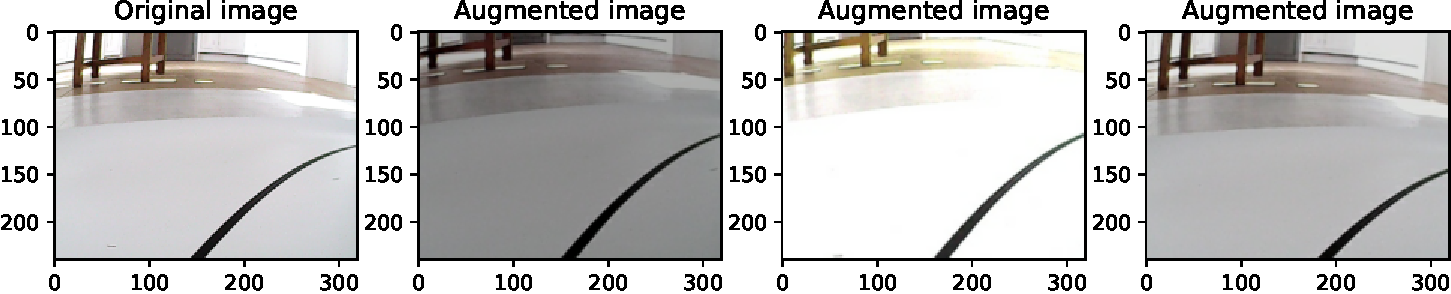
\includegraphics[width=0.9\textwidth]{figures/augmentation.pdf}
  \caption{Samples of augmented images.}
  \label{fig:augmentation}
\end{figure}

\paragraph{Data preprocessing}
\label{sec:data_preprocessing}
The image pixels were normalised to range of [-1, 1], matching the input range of the pre-trianed model.

\subsubsection{Modelling}
The steering angle model and the speed model were trained separately.

Transfer learning was used to train the models. The base model for both the steering angle and speed models was pre-trained on MobileNetV3Large, which provided a good balance between feature extracting complexity and efficiency. The base model was frozen to prevent overfitting. Each model was followed by 10 heads - sub-models that took the features extracted from the base model as the input and outputted the steering angle or speed. The use of varied head architectures aimed to capture diverse features from the images, thereby increasing model generalisability and improving prediction accuracy.

Figure \ref{fig:angle_heads} and Figure \ref{fig:speed_heads} show the structure of the heads.

\paragraph{Head's structures and hyperparameters}
\label{sec:structures_and_hyperparameters}

The head structures were randomly created using the constraints in Table \ref{tab:head_structure}. Dropout layers were added based on observed overfitting during training.

\begin{table}[H]
  \centering
  \renewcommand{\arraystretch}{1.2}
  \begin{tabular}{|l|l|}
    \hline
    \textbf{Component}       & \textbf{Configuration}                    \\
    \hline
    Convolutional layers     & 0 to 2                                    \\
    Pooling or flatten layer & One of: global average pooling or flatten \\
    Fully connected layers   & 0 to 4                                    \\
    Dropout                  & Added if overfitting was observed         \\
    \hline
  \end{tabular}
  \vspace{0.5em}
  \caption{Head structure configuration for model's heads.}
  \label{tab:head_structure}
\end{table}

The output layer of both the steering angle and speed models was a fully connected layer with one output with sigmoid activation, and the predicted values were the normalised steering angle and normalised speed respectively.

The hyperparameters of the layers in the models were chosen and tuned manually based on observed training and test loss.

\paragraph{Training}

The models were trained for 50 epochs with batch size of 64 and Adam optimiser with decaying learning rate:
\begin{equation}
  \begin{aligned}
    \text{learning\_rate} =
    \begin{cases}
      0.02,                                                                                                                                   & \text{if epoch = 0}
      \\
      \max\left(\frac{\text{initial\_learning\_rate}}{1 + \left(\frac{\text{epoch} - 1}{3}\right) \times \text{decay\_rate}}, 0.00015\right), & \text{otherwise}
    \end{cases}
    \\
    \text{where } \text{initial\_learning\_rate} = 0.01 \text{ and } \text{decay\_rate} = 0.4
  \end{aligned}
  \label{eq:learning_rate}
\end{equation}
This strategy kept the first epochs' learning rate high to improve convergence rate, while gradually decreased the learning rate to prevent overshooting.

Table \ref{tab:loss_functions} shows the loss functions used in training the models.

\begin{table}[h]
  \centering
  \renewcommand{\arraystretch}{1.2}
  \begin{tabular}{|l|l|}
    \hline
    \textbf{Model}       & \textbf{Loss function}      \\
    \hline
    Steering angle model & Mean squared error          \\
    Speed model          & Weighted mean squared error \\
    \hline
  \end{tabular}
  \vspace{0.5em}
  \caption{Loss functions used in training the models.}
  \label{tab:loss_functions}
\end{table}

The loss function's weights were calculated using inverse square root of the number of instances in each class:
\begin{equation}
  \text{weight}_c = \frac{1}{\sqrt{\text{number of instances in class}_c}}
  \label{eq:inverse_square_root}
\end{equation}
The resulting weights were then normalised so that the minimum weight was 1.

During the training of the steering angle models, the training data were randomly selected and augmented from the training set every epoch to reduce the risk of overfitting and introduce diversity of augmented images and undersampled classes.


\subsubsection{Prediction}
To further increase the generalisability of the predictions, 4 models were trained with different random seeds for the train/test split, and each image had \( 4 \times 10 = 40 \) predicted values for the steering angle and the speed. The predicted values were then averaged to obtain the prediction.

A threshold \(\text{speed}_\text{threshold}\) was introduced to the speed prediction to reduce the mean squared error (MSE) and was tuned using the test set. The speed prediction was adjusted as follows:

\begin{equation}
  \begin{aligned}
    \text{adjusted speed prediction} =
    \begin{cases}
      0.5 \times \operatorname{sign}(\tilde{y}) + 0.5, & \text{if } |\tilde{y}| > \text{speed}_\text{threshold} \\
      \tilde{y} + 0.5,                                 & \text{otherwise}
    \end{cases}
    \\
    \text{where } \tilde{y} = \text{original speed prediction} - 0.5
  \end{aligned}
\end{equation}

I manually inspected the predictions with high variance between the 40 predicted values to remove clearly incorrect predictions.



\begin{figure}[h]
  \centering
  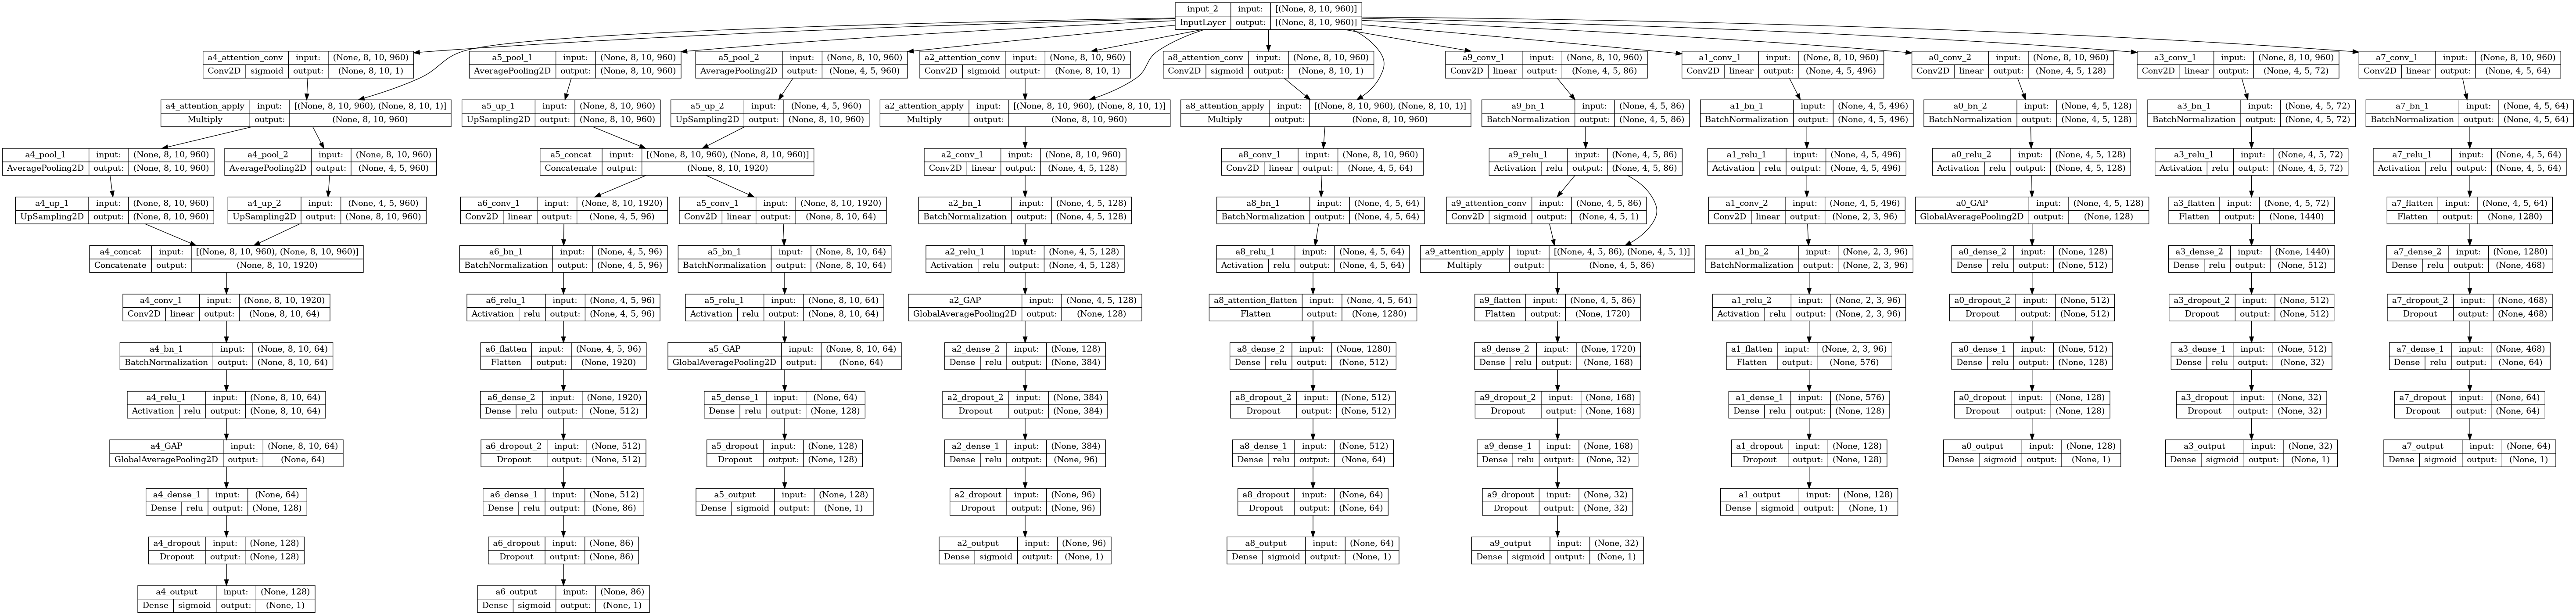
\includegraphics[width=0.9\textwidth]{figures/angle_heads.png}
  \caption{Structure of the steering angle model's heads.}
  \label{fig:angle_heads}
\end{figure}

\begin{figure}[h]
  \centering
  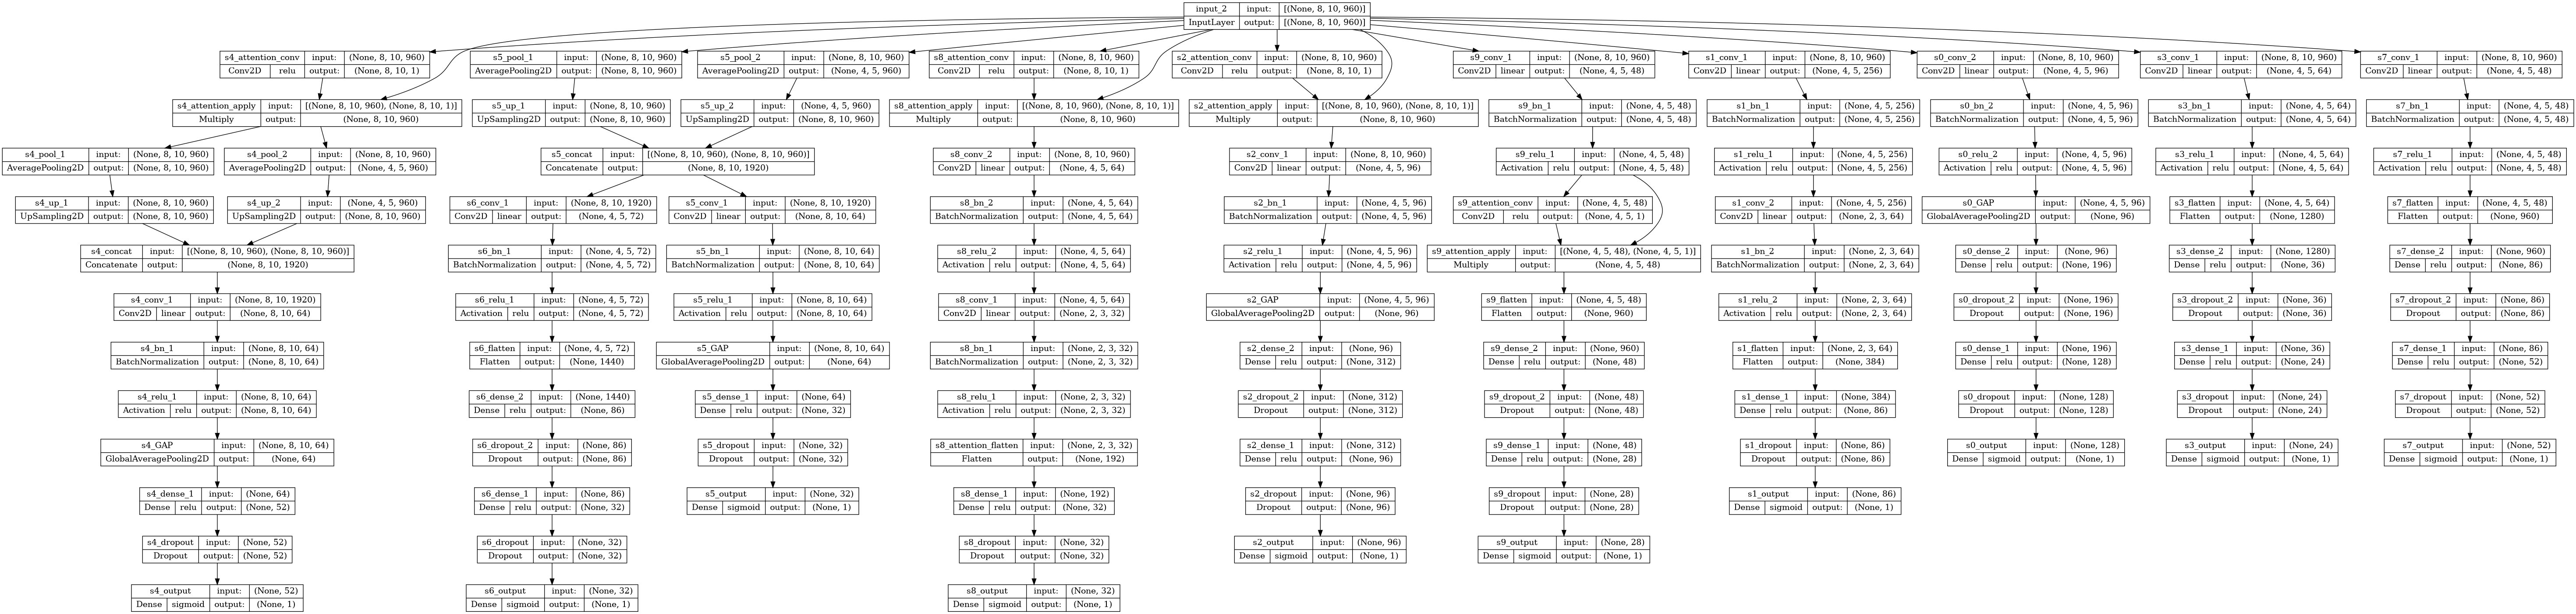
\includegraphics[width=0.9\textwidth]{figures/speed_heads.png}
  \caption{Structure of the speed model's heads.}
  \label{fig:speed_heads}
\end{figure}


\subsection{Live test}

The live test assessed the PiCar’s ability to complete tasks like lane following and stop when obstacles ahead on three maps - oval, figure-of-eight, and T-junction. The trained model was deployed.

\subsubsection{Training data}

\paragraph{Data collection and data cleaning}
To ensure consistent driving logic in the training data, 16.8k driving data were collected from scratch. The data were collected in the following ways:
\begin{itemize}
  \item Capture the PiCar's video feed and control signals while driving along all three maps in accordance with the rules outlined in \citep{Kaggle}.
  \item Train the model on the collected data and deploy the model to the PiCar.
  \item Additional data were collected to address the model's weak points. E.g.:
        \begin{itemize}
          \item Collect more data of turning left if the PiCar turned left poorly.
          \item Collect more data of stopping at a red light if the PiCar did not stop at a red light.
        \end{itemize}
  \item Retrain the model on the collected data and deploy the model to the PiCar.
  \item Repeat steps 3 and 4 until the PiCar achieved satisfactory performance.
\end{itemize}

The data were collected in batches. Data cleaning was performed after each batch by manually removing faulty or mislabelled images. Additional labels such as traffic light status and arrow direction were manually added. 

\paragraph{Data distribution}
The dataset is divided into four subsets: steering angle prediction, arrow prediction, "turn on arrow" prediction, and speed prediction. Arrow prediction identifies visible directional arrows, while "turn on arrow" prediction determines whether the PiCar should act on them. Figure \ref{fig:my_data_distribution} shows the collected data's distribution of each subset.

\begin{figure}[h]
  \centering
  \includegraphics[width=0.7\textwidth]{figures/my_data_distribution.pdf}
  \caption{Distributions of the collected data.}
  \label{fig:my_data_distribution}
\end{figure}

\paragraph{Training set and test set}
The dataset was split into training and test sets following the same method described in Section \ref{sec:train_test_split}.

\paragraph{Data balancing}
Data balancing was only applied to the training set.

The goal of this balancing was not only balancing the number of data in each class, but also balancing the number of data collected in each map, and balancing the importance of the data to the model. For example, I undersampled the data collected from the T-junction map for the angle model due to over-representation during reinforcement. Conversely, I oversampled the arrow classes to balance the number of data due to the rarity of appearing in the maps. I also undersampled the T-junction map data and oversampled the data that contained red light, green light, or objects for the speed model to improve the model's focus on these cases. Figure \ref{fig:my_data_distribution_after_balancing} shows the collected data's distributions after balancing.

\begin{figure}[h]
  \centering
  \includegraphics[width=0.7\textwidth]{figures/my_data_distribution_after_balancing.pdf}
  \caption{Distributions of the collected data after balancing.}
  \label{fig:my_data_distribution_after_balancing}
\end{figure}

The data for arrow prediction and "turn on arrow" prediction were left imbalanced because these two models were supportive models. They took care and overrode the steering angle output if the input image obviously contained arrows or the PiCar urgently needed to turn due to an arrow sign. These models were kept imbalanced to preserve their override role.

\paragraph{Data augmentation}
The data were augmented using the same method described in Section \ref{sec:data_augmentation}.

\paragraph{Data preprocessing}
The image size was halved from 240 x 320 to 120 x 160 to reduce the model's computational cost and inferencing time. Then the image pixels were normalised using the same method described in Section \ref{sec:data_preprocessing}.

\subsubsection{Modelling}
The four models were trained separately and shared the same base model, which was pre-trained on MobileNetV3Small, a model that is efficient for edge processing. They were then merged and converted into a TFLite model for deployment onto the PiCar.

The merged model used a shared untrainable backbone - from the input layer to the seventh layer from the end of the base model. The subsequent six layers (referred to as the neck) had the same structure but different weights. This shared feature extractor was followed by task-specific heads listed in Table \ref{tab:live_test_heads}.

\begin{table}[H]
  \centering
  \begin{tabular}{|c|c|}
    \hline
    \textbf{Head} & \textbf{Number of heads} \\ \hline
    \textbf{Steering angle head} & 3 \\ \hline
    \textbf{Arrow head} & 3 \\ \hline
    \textbf{"Turn on arrow" head} & 3 \\ \hline
    \textbf{Speed head} & 5 \\ \hline
  \end{tabular}
  \vspace{0.5em}
  \caption{Task-specific heads in the merged model.}
  \label{tab:live_test_heads}
\end{table}

Each task used multiple heads with slightly different structures to focus on slightly different features from the images to improve robustness.

Figure \ref{fig:live_test_heads} shows the structure of the merged model's heads.

\begin{figure}[h]
  \centering
  \includegraphics[width=0.95\textwidth]{figures/live_test_heads.png}
  \caption{Structure of the model's heads.}
  \label{fig:live_test_heads}
\end{figure}

\paragraph{Head's structures and hyperparameters}
The structures and the hyperparameters of the heads were mostly the same as described in Section \ref{sec:structures_and_hyperparameters}. However, the output layer of the speed model was changed to three output nodes with a Softmax activation to account for the three classes - normal, red light, and object ahead. The arrow and the "turn on arrow" models also had an output layer with 3 output nodes with a Softmax activation. The outputs represented left, right, or neither.

\paragraph{Training}
The models were trained for 40 epochs with frozen neck weights, batch size of 64, and Adam optimiser with decaying learning rate as described in Equation \ref{eq:learning_rate}. An additional 10 epochs were followed, with unfrozen neck weights. 

The models' loss functions were listed in Table \ref{tab:live_test_loss_functions}.

\begin{table}[H]
  \centering
  \begin{tabular}{|c|c|}
    \hline
    \textbf{Model} & \textbf{Loss function} \\ \hline
    \textbf{Steering angle model} & Mean squared error \\ \hline
    \textbf{Arrow model} & Weighted cross-entropy \\ \hline
    \textbf{"Turn on arrow" model} & Weighted cross-entropy \\ \hline
    \textbf{Speed model} & Weighted cross-entropy \\ \hline
  \end{tabular}
  \vspace{0.5em}
  \caption{Loss functions of the models.}
  \label{tab:live_test_loss_functions}
\end{table}

The loss functions' class weights were calculated using inverse square root of the number of instances in each class, as shown in Equation \ref{eq:inverse_square_root}. The resulting weights were then normalised so that the minimum weight within each model's set of weights was 1.

\subsubsection{Prediction}
Predictions were obtained by averaging.

The output steering angle was adjusted as follows:
\begin{itemize}
  \item If left arrow and turn on left arrow were predicted, the steering angle was set to 0.
  \item If right arrow and turn on right arrow were predicted, the steering angle was set to 1.
  \item Otherwise, the steering angle was adjusted based on the predicted steering angle:
        \begin{equation}
          \begin{aligned}
            \text{output}_{\text{steering angle}} =
            \begin{cases}
              \hat{y}_{\text{angle}},                                                                    & \text{if } \left| \hat{y}_{\text{angle}} - 0.5 \right| < 0.01 \\
              \operatorname{clip}\left( (\hat{y}_{\text{angle}} - 0.5) \times 1.3,\ -0.5,\ 0.5 \right) + 0.5, & \text{otherwise}
            \end{cases}
            \\
            \text{where } \hat{y}_{\text{angle}} \text{ is the predicted steering angle.}
          \end{aligned}
        \end{equation}
        The above adjustment increased the steering response to sharper turns to compensate understeering issues of the PiCar observed in the deployment and testing.
\end{itemize}
The output speed was set to 1 if the speed prediction is normal. Otherwise, the output speed was 0.


\section{Results}

\subsection{Online challenge}
The final model achieved MSEs of 0.00917 and 0.01127 on the public and private leaderboards respectively, ranked first on both.

In the training phase, the speed model achieved an MSE of 0.0073 and 0.0103 on the training and test set respectively. Figure \ref{fig:speed_model_eval} and \ref{fig:angle_model_error} shows evaluation results on the test set.


\begin{figure}[h]
  \centering
  \begin{subfigure}[b]{0.48\textwidth}
    \includegraphics[width=\textwidth]{figures/speed_cm.pdf}
    \caption{Confusion matrix for the speed model predicting on the test set.}
    \label{fig:speed_cm}
  \end{subfigure}
  \hfill
  \begin{subfigure}[b]{0.48\textwidth}
    \includegraphics[width=\textwidth]{figures/speed_throshold_vs_mse.pdf}
    \caption{MSE vs. threshold for the speed model predicting on the test set.}
    \label{fig:speed_throshold_vs_mse}
  \end{subfigure}
  \caption{Evaluation results of the speed model on the test set.}
  \label{fig:speed_model_eval}
\end{figure}

\begin{figure}[h]
  \centering
  \includegraphics[width=0.95\textwidth]{figures/angle_model_error.pdf}
  \caption{Box plot and violin plot of one of the angle model's error on the test set.}
  \label{fig:angle_model_error}
\end{figure}



\subsection{Live test}
Table \ref{tab:live_test_model_losses} shows the training and test metrics of randomly picked heads of the steering angle and speed model in the training phase.
\begin{table}[h]
  \centering
  \renewcommand{\arraystretch}{1.3}
  \begin{tabular}{|c|c|c|c|}
    \hline
    \textbf{Model}       & \textbf{Metric}         & \textbf{Training} & \textbf{Test} \\
    \hline
    \textbf{Angle model} & Mean square error (MSE) & 0.0055            & 0.0046        \\
    \hline
    \textbf{Speed model} & Balanced accuracy       & 98.85\%           & 99.32\%       \\
    \hline
  \end{tabular}
  \vspace{0.5em}
  \caption{Training and test metrics of randomly picked heads of the steering angle and speed model in the training phase.}
  \label{tab:live_test_model_losses}
\end{table}

On the live test day, 69.4\% of the tasks were completed successfully. As shown in Table \ref{tab:live_test_day_performance}, the model excelled in lane following and object detection, but show weaknesses in interpreting traffic light signals and arrow signs.

\begin{table}[h]
  \centering
  \renewcommand{\arraystretch}{1.3}
  \begin{tabular}{|c|c|}
    \hline
    \textbf{Task}                         & \textbf{Performance} \\
    \hline
    \textbf{Lane following}               & Flawless             \\
    \hline
    \textbf{Drive when the road is clear} & Needs improvement    \\
    \hline
    \textbf{Stop on object}               & Flawless             \\
    \hline
    \textbf{Stop at traffic light}        & Poor                 \\
    \hline
    \textbf{Responding to arrow signs}    & Inconsistent         \\
    \hline
  \end{tabular}
  \vspace{0.5em}
  \caption{Model performance in different categories on the live test day.}
  \label{tab:live_test_day_performance}
\end{table}


\section{Discussion}

\subsection{Performance reflection on metrics}
\label{sec:performance_reflection_on_metrics}
In the online challenge, the model's MSE remained constantly low across the training set, test set, and both public and private leaderboard, indicating strong generalisability and minimal overfitting.

In the live test parse, the model performed better in the test set than on the training set, suggesting strong generalisability and minimal overfitting. During the training parse, data augmentation - such as cropping and rotating - was applied to the training set to reduce overfitting. However, this sometimes led to the loss of important features at the edges or corners of images, confusing the model. For example, in some "red light" images, a traffic light appeared near the edge of the frame. After augmentation, the traffic light was cropped and lost, creating a mismatch between the image and its label. In the future, less aggressive augmentation could be used to preserve critical features and prevent the problem.

\subsection{Error analysis}

\subsubsection{Speed predictions}
The model performed poorly on the tasks "drive when the road is clear" and "stop at traffic light". Gradient-weighted class activation map (Grad CAM) was carried to investigate potential causes. Figure \ref{fig:gradcam_result} shows the results on several red light and green light images. Subfigures \subref{fig:gradcam_result_1}, \subref{fig:gradcam_result_2}, and \subref{fig:gradcam_result_3} illustrate that the model focused on irrelevant features - such as the side of the road and the traffic light's wire - when detecting red light. In contrast, subfigures \subref{fig:gradcam_result_4} and \subref{fig:gradcam_result_5} show that the model was able to correctly focus on the green light and classify the speed output as normal. However, Figure \ref{fig:gradcam_result_6} shows a case where the model focused on the road but classified the image as containing red light.

As discussed in \ref{sec:performance_reflection_on_metrics}, one likely cause is the use of aggressive augmentation. Cropping and rotating the images may have removed key features - such as traffic lights near the edges or corners - leading to mislabelled training samples. For instance, if an image was labelled "red light" but the augmentation cropped out the traffic light located at the edge of the image, the model may have learned to rely on irrelevant background cues.

To address this, first, less aggressive augmentation - particularly cropping - could be used to preserve important context. Second, manual filtering the dataset could be performed to remove samples in which critical features appear at the image boundaries. This would allow more aggressive augmentation strategies to be retained without compromising label quality.

\begin{figure}[h]
  \centering

  \begin{subfigure}[t]{0.3\textwidth}
    \centering
    \includegraphics[width=\linewidth]{figures/gradcam_result_1.pdf}
    \caption{Grad CAM result on a red light image.}
    \label{fig:gradcam_result_1}
  \end{subfigure}
  \hfill
  \begin{subfigure}[t]{0.3\textwidth}
    \centering
    \includegraphics[width=\linewidth]{figures/gradcam_result_2.pdf}
    \caption{Grad CAM result on a red light image.}
    \label{fig:gradcam_result_2}
  \end{subfigure}
  \hfill
  \begin{subfigure}[t]{0.3\textwidth}
    \centering
    \includegraphics[width=\linewidth]{figures/gradcam_result_3.pdf}
    \caption{Grad CAM result on a red light image.}
    \label{fig:gradcam_result_3}
  \end{subfigure}

  \vspace{1em} % Space between rows

  \begin{subfigure}[t]{0.3\textwidth}
    \centering
    \includegraphics[width=\linewidth]{figures/gradcam_result_4.pdf}
    \caption{Grad CAM result on a green light image.}
    \label{fig:gradcam_result_4}
  \end{subfigure}
  \hfill
  \begin{subfigure}[t]{0.3\textwidth}
    \centering
    \includegraphics[width=\linewidth]{figures/gradcam_result_5.pdf}
    \caption{Grad CAM result on a green light image.}
    \label{fig:gradcam_result_5}
  \end{subfigure}
  \hfill
  \begin{subfigure}[t]{0.3\textwidth}
    \centering
    \includegraphics[width=\linewidth]{figures/gradcam_result_6.pdf}
    \caption{Grad CAM result on a green light image.}
    \label{fig:gradcam_result_6}
  \end{subfigure}

  \caption{Grad CAM results on red light and green light images.}
  \label{fig:gradcam_result}
\end{figure}


\subsubsection{Arrow signs behaviour}

The model performed inconsistently in classifying left, right, or no arrows. Grad CAM was used to investigate potential causes. Figure \ref{fig:gradcam_arrow} shows the Grad CAM results on images with arrows. Subfigures \subref{fig:gradcam_left_1}, \subref{fig:gradcam_left_2}, \subref{fig:gradcam_left_3} and \subref{fig:gradcam_right_2} demonstrate that although the model correctly predicted, it often focused on irrelevant regions such as the background or the edge of the image. In contrast, subfigure \subref{fig:gradcam_right_1} shows the model attending to the key feature and predicted correctly. Subfigure \subref{fig:gradcam_right_3}, however, illustrates a case where the model focused on some relevent features but still predicted wrongly.

This inconsistency may be due to the model's difficulty in capturing and distinguishing left and right arrows. To further examine this, a binary classification model was trained specifically to distinguish left/right arrows. It achieved a balanced accuracy of 0.95 on the training set but only 0.83 on the test set, suggesting limited generalisability. Combined with the Grad CAM result, this indicates that the model - with image size of 120 x 160 and MobileNetV3Small backbone - may have overfitted to contextual background features rather than learning robust arrow representation of the arrow shape. The low image resolution may be a contributing factor. However, due to the limited computational power on the PiCar, increasing image resolution would significantly increase inference time, resulting in high latency in car control decisions.


\begin{figure}[h]
  \centering

  \begin{subfigure}[t]{0.3\textwidth}
    \centering
    \includegraphics[width=\linewidth]{figures/gradcam_left_1.pdf}
    \caption{Grad CAM result on a left arrow image.}
    \label{fig:gradcam_left_1}
  \end{subfigure}
  \hfill
  \begin{subfigure}[t]{0.3\textwidth}
    \centering
    \includegraphics[width=\linewidth]{figures/gradcam_left_2.pdf}
    \caption{Grad CAM result on a left arrow image.}
    \label{fig:gradcam_left_2}
  \end{subfigure}
  \hfill
  \begin{subfigure}[t]{0.3\textwidth}
    \centering
    \includegraphics[width=\linewidth]{figures/gradcam_left_3.pdf}
    \caption{Grad CAM result on a left arrow image.}
    \label{fig:gradcam_left_3}
  \end{subfigure}

  \vspace{1em} % Space between rows

  \begin{subfigure}[t]{0.3\textwidth}
    \centering
    \includegraphics[width=\linewidth]{figures/gradcam_right_1.pdf}
    \caption{Grad CAM result on a right arrow image.}
    \label{fig:gradcam_right_1}
  \end{subfigure}
  \hfill
  \begin{subfigure}[t]{0.3\textwidth}
    \centering
    \includegraphics[width=\linewidth]{figures/gradcam_right_2.pdf}
    \caption{Grad CAM result on a right arrow image.}
    \label{fig:gradcam_right_2}
  \end{subfigure}
  \hfill
  \begin{subfigure}[t]{0.3\textwidth}
    \centering
    \includegraphics[width=\linewidth]{figures/gradcam_right_3.pdf}
    \caption{Grad CAM result on a right arrow image.}
    \label{fig:gradcam_right_3}
  \end{subfigure}

  \caption{Grad CAM results on arrow images.}
  \label{fig:gradcam_arrow}
\end{figure}




\subsection{Design decisions}
In the online challenge, multiple multi-head models were used to produce the final prediction. Each head had a slightly different structure, allowing for a more diverse interpretation of the extracted feature from the shared pre-trained backbone. Additionally, training multiple models on different subsets of the training data further increased the diversity of the learned representations. These choices improved generalisability and accuracy stability.

In the live test model, a smaller pre-trained base model was chosen to reduce the inferencing time on the Raspberry Pi (RPi) single-board computer. This improved the reliability of real-time processing by providing more computational headroom, helping to counter the fluctuating inference speed - which occasionally ranged from 70 ms to 150 ms despite the CPU not being fully utilised or thermally throttled. Combining the models into a multi-head architecture with a shared backbone, and converting resulted model into a TFLite model for deployment on the PiCar, also improved inferencing efficiency.

\subsection{Iterative data collection in live test phase}
The iterative data collection during the live test phase helped reinforce the model's weaknesses by targeting the failure cases observed during deployment. For example, if the PiCar failed to stop at the red lights or struggled to detect pedestrians ahead, additional data were collected specifically for those scenarios. This approach improved the model's robustness and allowed it to generalise better across edge cases. However, these reinforcements altered the previous dataset's class distribution, requiring the data balancing parameters to be re-tuned after each iteration.

\subsection{Directions of further study}
Control signals depend on both current and previous frames. Future studies could incorporate previous frames' information into the model using recurrent neural network (RNN) structures or long short-term memory (LSTM) layers. This may help the model better understand motion patterns, anticipate upcoming turns, and make smoother and more accurate control decisions.

Another promising direction is to equip the PiCar with an additional camera to enable stereo vision. This would allow the system to acquire depth information, which could significantly improve its ability to detect and respond to road signs, objects, and pedestrians in 3D space.

\section{Conclusion}
This project developed and deployed machine learning models to predict steering angle and speed from PiCar's camera input using transfer learning. The model achieved strong performance in the online challenge and successfully completed most live test tasks, though remain in red light detection and arrow classification. Future work could improve generalisability and accuracy through enhanced data collection and integration of sequential modelling.


\bibliographystyle{plainnat}  % or use abbrvnat, unsrtnat, etc.
\bibliography{references}



\end{document}